\section{\fontsize{20}{0}{\selectfont{Metodolog�a}}}
\rule{\textwidth}{1pt}\\

En esta secci�n se describen las herramientas, estrategias, t�cnicas y procedimientos requeridos para satisfacer el objetivo principal del proyecto y llegar a una soluci�n de la problem�tica. El desarrollo de esta se asume tratando individualmente cada objetivo espec�fico detallando las actividades necesarias para su total cumplimiento. Las fases para el desarrollo del poyecto se observan en la Figura \ref{meto}.
\begin{figure}[H]
	\centering
	\shadowbox{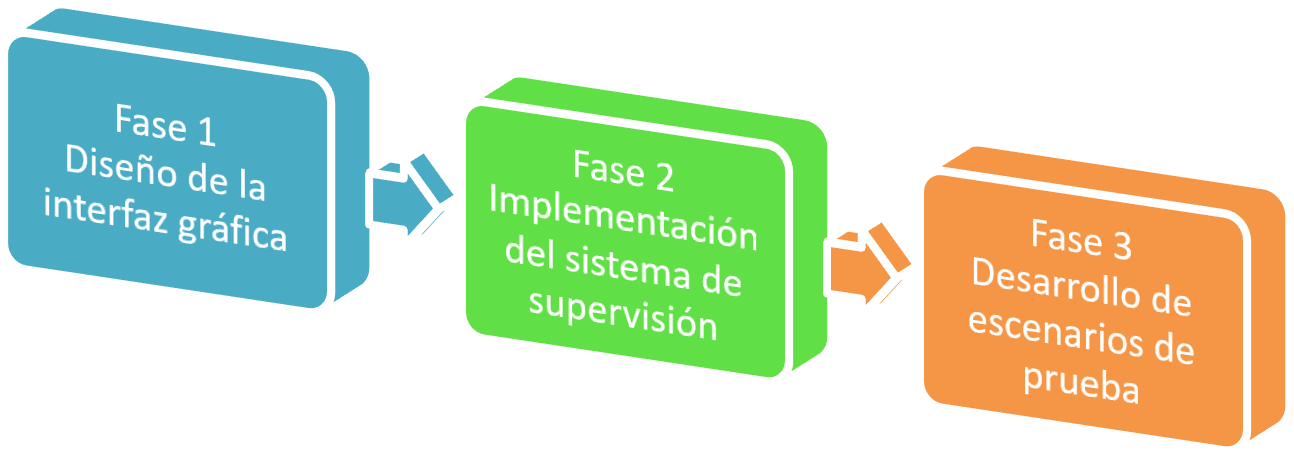
\includegraphics[width=0.88\textwidth]{meto}}
	\caption{Fases para el desarrollo del proyecto}
	\label{meto}
\end{figure}
En la primera fase se definir� la plataforma en la cual se dise�ar� la interfaz gr�fica ya sea escritorio, web, Android, IOS u otra. Posteriormente, se realizar� la revisi�n de los diferentes lenguajes de programaci�n que pueden ser empleados para la elaboraci�n de la interfaz gr�fica de acuerdo con el entorno anteriormente establecido, para finalmente profundizar en los diferentes conceptos y herramientas disponibles del lenguaje en cuesti�n para la elaboraci�n de la primera versi�n de la interfaz.\\

Una vez dise�ada la parte gr�fica (est�tica de la aplicaci�n) en la segunda fase se dise�ar� un modelo en 3D de la estaci�n de supervisi�n con el fin de incluirla dentro de la aplicaci�n para posteriormente realizar la vinculaci�n del nodo central de la red y la interfaz gr�fica con un servidor com�n en la nube para la lectura de datos y manipulaci�n de los diferentes sensores la red inal�mbrica WSN (Wireless Sensor Networks) a trav�s de internet.\\

Finalmente, en la �ltima fase se plantear�n diversas pruebas de lectura y manipulaci�n de los diferentes nodos de la red en un entorno local, con el fin de identificar los fallos (bugs) presentados, esto con el objetivo de realizar la oportuna correcci�n de hardware o software (seg�n sea el caso) para as�, obtener un correcto funcionamiento de la red. Con las pruebas locales superadas se proceder� a realizar una prueba final de toda la red de sensores de manera remota para verificar su correcto funcionamiento.\\

Al terminar cada una de las fases anteriormente mencionadas se realizar� la creaci�n de un manual de usuario y cartilla de implementaci�n para todo el sistema completo, esto con el objetivo de capacitar a la comunidad externa y acad�mica interesada. Adem�s, se desarrollar� un documento para participaci�n en eventos cient�ficos.

\newpage